%!TEX root = ../master.tex
\section{Electrical company attacking the consumer}
The electrical company sells electricity to the consumer as a service.
Some electrical companies may want to raise the earnings by charging the consumer more than they actually have consumed for.
In order to make it difficult for the consumer to detect the changes the electrical company needs to make the bill and the amount reported by the smart meter identical.
It is therefore necessary to compromise the smart meter.

\paragraph{Gaining access}
The attack tree for this scenario can be seen on \cref{electrical_vs_consumer}.
\Cref{compromise:SM} describes how to compromise the smart meter.
The electrical company has more limited possibilities than described, because logging into the smart meter does not give the electrical company any advantage in earning more money.

\paragraph{Altering the consumption}
When access is gained the electrical company can abuse the attained power to change the actual data on the smart meter.
This data is then later sent to the Data Hub and the electrical company will calculate the bill as if nothing happened.

A slightly different option is to bribe the smart meter manufacturer into changing how the smart meter stores consumption data.
If the smart meter records a slightly higher value than actually measured, the electrical company will benefit greatly from rolling that firmware out to thousands of users.
This method is also more transparent because the consumer will have a reported consumption that is only slightly higher than expected, and it will therefore be harder for the consumer to recognize.

\begin{figure}
  \begin{center}
    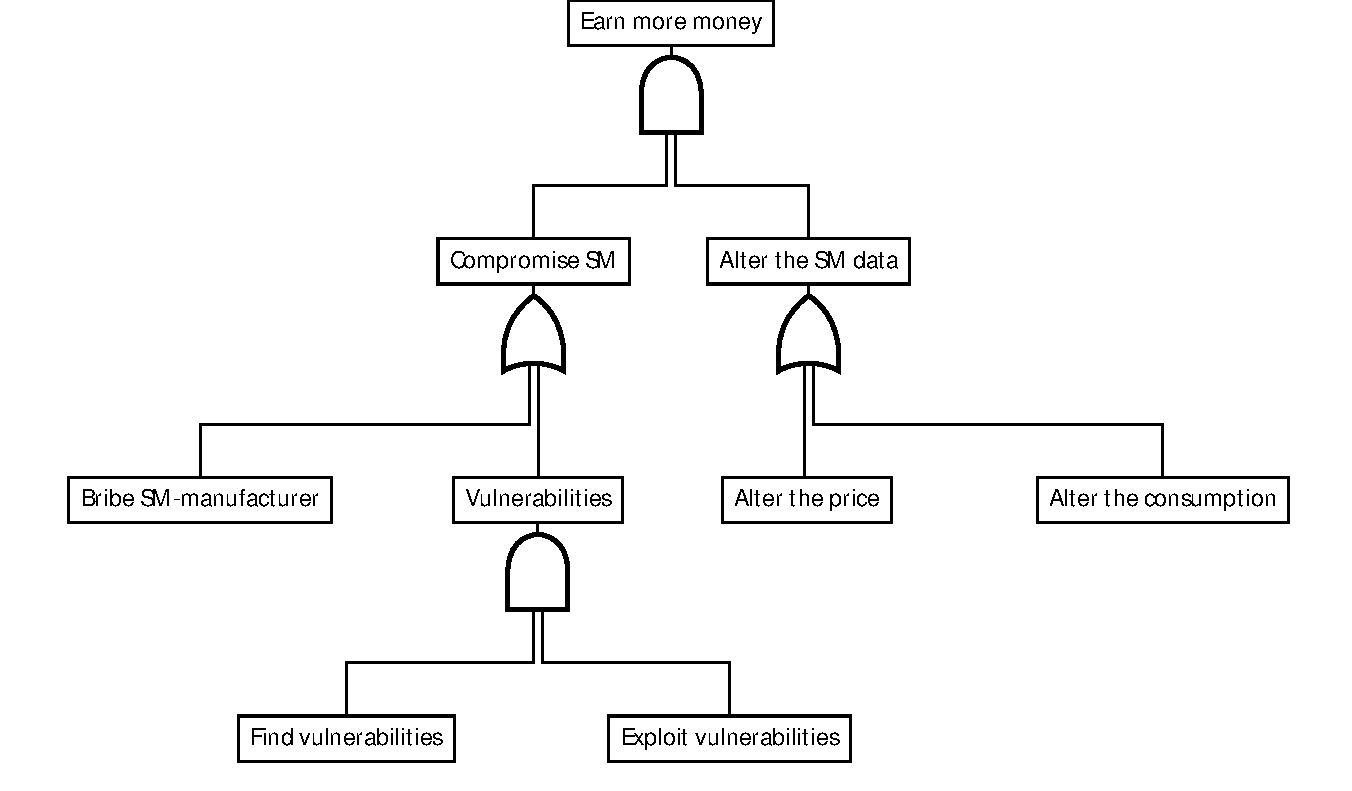
\includegraphics[ width=\textwidth]{graphviz/electrical_company_vs_consumer.pdf}
  \end{center}
  \caption{The electrical company attacking the consumer.}
  \label{electrical_vs_consumer}
\end{figure}
